%%%%%%%%%%%%%%%%%%%%%%%%%%%%%%%%%%%%%%%%%
% Short Sectioned Assignment
% LaTeX Template
% Version 1.0 (5/5/12)
%
% This template has been downloaded from:
% http://www.LaTeXTemplates.com
%
% Original author:
% Frits Wenneker (http://www.howtotex.com)
%
% License:
% CC BY-NC-SA 3.0 (http://creativecommons.org/licenses/by-nc-sa/3.0/)
%
%%%%%%%%%%%%%%%%%%%%%%%%%%%%%%%%%%%%%%%%%

%----------------------------------------------------------------------------------------
%	PACKAGES AND OTHER DOCUMENT CONFIGURATIONS
%----------------------------------------------------------------------------------------

\documentclass[paper=a4, fontsize=11pt]{scrartcl} % A4 paper and 11pt font size

\usepackage[T1]{fontenc} % Use 8-bit encoding that has 256 glyphs
\usepackage{fourier} % Use the Adobe Utopia font for the document - comment this line to return to the LaTeX default
\usepackage[english]{babel} % English language/hyphenation
\usepackage{amsmath,amsfonts,amsthm} % Math packages

\usepackage{lipsum} % Used for inserting dummy 'Lorem ipsum' text into the template

\usepackage{sectsty} % Allows customizing section commands
\allsectionsfont{\centering \normalfont\scshape} % Make all sections centered, the default font and small caps

\usepackage{tikz}
\usetikzlibrary{plotmarks}

\usepackage{enumitem}
\usepackage{lastpage}
\usepackage{multirow}
\usepackage{fancyhdr} % Custom headers and footers
\pagestyle{fancyplain} % Makes all pages in the document conform to the custom headers and footers
\fancyhead{} % No page header - if you want one, create it in the same way as the footers below
\fancyfoot[L]{} % Empty left footer
\fancyfoot[C]{} % Empty center footer
\fancyfoot[C]{\thepage~of~\pageref{LastPage}} % Page numbering for right footer
\renewcommand{\headrulewidth}{0pt} % Remove header underlines
\renewcommand{\footrulewidth}{0pt} % Remove footer underlines
\setlength{\headheight}{13.6pt} % Customize the height of the header

\setlength\parindent{0pt} % Removes all indentation from paragraphs - comment this line for an assignment with lots of text

%----------------------------------------------------------------------------------------
%	TITLE SECTION
%----------------------------------------------------------------------------------------

\newcommand{\horrule}[1]{\rule{\linewidth}{#1}} % Create horizontal rule command with 1 argument of height



\title{	
\normalfont \normalsize 
\textsc{Norwegian University of Science and Technology\\TDT4200 -- Parallel Computing} \\ [25pt]
\horrule{0.5pt} \\[0.4cm]
\huge Problem Set 2:\\ CUDA Intro\\
\horrule{2pt} \\[0.5cm]
}

\author{Per Magnus Veierland\\permve@stud.ntnu.no}

\setlist[enumerate,1]{label=\emph{\alph*})}
\setlist[enumerate,2]{label=\roman*)}
\setlist[enumerate,3]{label=\arabic*)}

\date{\normalsize\today}

\newacro{CPU}{Central Processing Unit}
\newacro{CUDA}{Compute Unified Device Architecture}
\newacro{GPU}{Graphics Processor Unit}
\newacro{MIMD}{Multiple Instruction Multiple Data}
\newacro{NUMA}{Nonuniform memory access}
\newacro{SGI}{Silicon Graphics International}
\newacro{SIMT}{Single Instruction Multiple Thread}
\newacro{SMT}{Simultaneous Multi-threading}
\newacro{SM}{Streaming Multi-processor}
\newacro{UMA}{Uniform memory access}

\begin{document}
\maketitle

\section*{Part 1: Theory}

\subsection*{Problem 1: Problem 1, Architectures \& Programming Models}

\begin{enumerate}

\item \textbf{Briefly explain the differences between the following architectures:\\
Keywords being: Homogeneous cores, heterogeneous cores, clusters, NUMA, threads.}

\begin{enumerate}
\item \textit{Nvidia Maxwell} is the latest generation \ac{GPU} architecture from Nvidia. Their \ac{GPU} architecture is highly parallel, with a chip such as the GM204 having 16 \acp{SM} split into 4 distinct \ac{CUDA} processing blocks, each containing 32 homogeneous \ac{CUDA} cores. In total the GM204 chip has 2048 \ac{CUDA} processing cores.

Within each \textit{processing block} (not to be mixed with \textit{thread block}) there is a register file which is shared by the processing cores and is used for thread register storage and thread local storage. All processing blocks within an \ac{SM} has one L1/texture cache as well as a shared memory. All \acp{SM} share a common L2 cache. There is no L3 cache. For each memory; the thread private memory, the \ac{SM} shared memory, and the external global memory; there is equal access time for all users, so the architecture has uniform memory access.

Threads in a \ac{CUDA} system are used to execute kernel programs. Each thread has its own program counter, registers and thread local storage. This data is stored in the processing block's register file. Threads are organized into \textit{thread blocks} by the application. The \ac{GPU} global \textit{GigaThread Engine} schedules thread blocks onto \acp{SM}. Within an \ac{SM} threads are executed as part of warps. A \textit{warp} is a collection of 32 threads which is executed simultaneously. The GM204 chip has 4 \textit{warp schedulers} per \ac{SM} which each can dispatch two instructions per warp per clock cycle. Since there is no register state within the processing cores, only in the register file, the \ac{SM} can immediately switch between executing different warps without any context switch cost. When executing a warp every processing core must execute the same instruction. This is what makes the architecture \ac{SIMT}; there is a single instruction being executed by multiple threads simultaneously. 

\item \textit{ARM big.LITTLE} is a heterogeneous computer architecture consisting of a set of smaller (``little'') processing cores combined with a set of larger (``big'') processing cores. The architecture is primarily intended for embedded applications, especially smartphones, where power consumption is of great concern. Having smaller cores with less functionality which can used to handle lighter tasks saves the system from spending more power to achieve the same task with a bigger, more power demanding processing core. The memory access is uniform. 

The \textit{ARM big.LITTLE} can be viewed and used as being composed of two clusters, the ``high'' cluster consisting of the ``big'' cores, and the ``low cluster'' consisting of the ``little'' cores. With clustered switching, only one of the clusters is used a time and the operating system can only view and use one cluster at a time. The processor cores share access to the L2 cache which is used to transfer state when switching execution between the two clusters.

\item \textit{Vilje @ NTNU} is a \ac{SGI} Altix ICE X system composed of a cluster of 1404 nodes connected by an Infiniband interconnect which is used for communication between nodes.

Each node in the system consists of two Intel Xeon ``Sandy Bridge'' processors bridged with an Intel QuickPath interconnect. Both processors has a separate 16~GB memory which they can access directly. In addition, each processor can access the memory connected to the other processor through the Intel QuickPath interconnect. This makes it a \ac{NUMA} architecture. The advantage is that each processor can access their own memory faster they would be able to access a single shared memory used by both processors; while still being able to take advantage of shared-memory programming by having access to the other processor's memory as well.

The Intel Xeon E5-2670 processors used for each node has eight homogeneous cores each for a total of 16 processing cores per node. Each processing core has a dedicated L1 (32~KB) and L2 (256~KB) cache. The L3 (20~MB) cache is shared between all cores in the processor.

The processor cores supports \ac{SMT}, also known by the term \textit{Hyper-threading} used by Intel, which allows a single physical processor core to simultaneously execute two logical threads. This is possible because each processor core is able to hold the state for two threads simultaneously and weaves their execution through a shared instruction pipeline. This technique helps the processor core better utilize all of its functional units, leading to more efficient execution.

\item \textit{A Typical modern-day \ac{CPU}} consists of one physical processor with 2-8 homogeneous cores and uniform memory access. Most often each core will support \ac{SMT} also known as \textit{Hyperthreading} for Intel processors which allows each core to execute two threads in one instruction pipeline. A modern \ac{CPU} typically has 3 on-chip caches known as the L1, L2, and L3 cache. The processor cores are usually quite sophisticated and contains functionality for pipelining with branch prediction, speculative execution as well as predicting memory access and pre-fetching data from memory. A single \ac{CPU} system, although it has multiple cores, is not usually viewed as a cluster.

\end{enumerate}

\item \textbf{Explain Nvidia's SIMT addition to Flynn's Taxonomy, and how it is realized, if at all, in each of the architectures from a).}

\acf{SIMT} is used by Nvidia to describe an architecture where a single instruction stream is executed in parallel for a set of threads. This is realized by having ``warps'' of threads execute on a \acf{SM} which has one instruction decoder for a large set of functional cores. This allows a single instruction to be executed in exact parallel for a set of threads.

The \textit{Nvidia Maxwell} architecture implements \ac{SIMT} through having a set of \acp{SM}, each with four warp schedulers. Each \ac{SM} has a large number of cores which each warp scheduler uses to execute sets of threads.

None of the other architectures mentioned in a) implements \ac{SIMT}. \ac{SMT} / \textit{Hyperthreading} is different as it involves multiple instruction streams and does not perform simultaneous computation.

\item \textbf{For each architecture from a), report which classification from Flynn's Taxonomy is best suited. If applicable, also state if the architecture fits Nvidia's SIMT-classification. Give the reasoning(s) behind your answers.}

\begin{itemize}

\item
\textit{Nvidia Maxwell} can be described as both \ac{SIMT} and \ac{MIMD}. The \ac{SIMT} description is used to describe how warps are executed on the \ac{GPU} architecture, where a single instruction stream is shared by many threads with different data. A \ac{SIMT} architecture by definition operates on multiple data streams. However since Maxwell systems has several \acp{SM}, each capable of executing multiple kernels in parallel with different instruction streams, the system as a whole can also be described as having multiple instruction streams, thus being a \ac{MIMD} system as well.

\item
\textit{ARM big.LITTLE} can be described as a \ac{MIMD} system as it has multiple processing cores executing multiple instruction streams, and since it supports vector instructions allowing it to work on multiple data streams. It can not be described as a \ac{SIMT} architecture.

\item
\textit{Vilje @ NTNU} can be described as being a \ac{MIMD} systems, both on a ``low level'' since it runs on processors with multiple cores supporting vector instructions -- and on a ``higher level'' since it is a clustered system where different instruction streams are run on different processors with different data. It can not be described as a \ac{SIMT} system.

\item
\textit{A typical modern-day \ac{CPU}} can be described as a \ac{MIMD} system since it consists of multiple processing cores capable of executing multiple instruction streams in parallel on separate sets of data. It also supports vector instructions which would make each processor core capable of multiple data stream usage. It can not be described as a \ac{SIMT} system.

\end{itemize}

\end{enumerate}

\subsection*{Problem 2: CUDA GPGPUs}

\begin{enumerate}

\item \textbf{Explain the terms \textit{Threads}, \textit{Grids}, \textit{Blocks}, and how they relate to one another (if at all).}

\begin{itemize}

\item In a \ac{CUDA} architecture a \textit{thread} represents one distinct execution of a kernel. A kernel is a general-purpose program running on the \ac{GPU} and can be executed by a large number of threads simultaneously. Each thread has its own registers, program counter and private memory. 

\item A \textit{block} is a collection of threads executing the same kernel on a single \ac{SM}. Each block has a very fast local memory which the threads within the block can use to exchange data. Blocks can be executed in any order. All threads in a block will not necessary execute at the same time; see the description of warps in the answer to question \textit{2d}. Threads in a block can synchronize their execution with a special barrier mechanism.

The \textit{number of threads per block} is specified at runtime when launching a kernel. As a convenience it is implemented as a 3-dimensional vector, where the threads for each block can be organized into 1, 2, or 3 dimensions according to what best describes the problem. The built-in variable \texttt{threadIdx} has a unique value available to each \ac{CUDA} thread specifying its \textit{X-Y-Z} index within the block. The built-in variable \texttt{blockDim} specifies the dimensions of the block.

For Maxwell, the maximum number of threads per block is $1024$, the maximum number of threads in the X-dimension for a block is $2^{32}-1$, and the maximum number of threads in the Y- and Z-dimensions is $65535$.

\item When launching a kernel, both the \textit{number of blocks} and the \textit{number of threads per block} is specified at runtime. The set of blocks instantiated for a launched kernel is known as a \textit{grid}.

The \textit{number of blocks} is also given as a 3-dimensional which can be used according to what best describes the problem. The built-in variable \texttt{blockIdx} provides the \textit{X-Y-Z} index of the block which a \ac{CUDA} thread is a part of. The built-in variable \texttt{gridDim} specifies the dimensions of the associated grid.

For Maxwell, the maximum number of blocks in the X- and Y-dimension of a grid is $1024$, and the maximum number of blocks in the Z-dimension of a grid is $64$.

\end{itemize}

Figure \ref{figure:gridblock} shows that a \textit{block} is composed of a set of \textit{threads}, that a \textit{grid} is composed of a set of \textit{blocks}, and that there is a separate \textit{grid} per \textit{kernel} executed on the \textit{device}.

\begin{figure}[p]
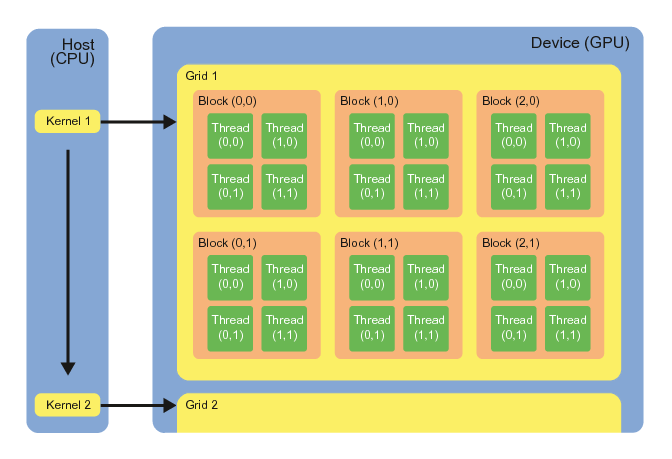
\includegraphics[width=\linewidth]{images/gridblock}
\caption{Organizational view showing how kernels, grids, blocks and threads are related in a \ac{CUDA} \ac{GPU} architecture. Source: ``Performance potential for simulating spin models on GPU'' by Martin Weigel 2011 (http://inspirehep.net/record/883697?ln=en).}
\label{figure:gridblock}
\end{figure}

\item \textbf{Consider an algorithm whose input has size $2n$, output has size $5n$, and execution time is $5hn \cdot 7h \cdot \log_2(n)$ where $h = 1$ on the GPU and $h = 10$ on the \ac{CPU}. The ac{CPU}-GPU bus has a bandwidth of $r$. How big must $n$ be before it is faster to run the dataset with the algorithm detailed on the GPU instead of the ac{CPU}?}

When comparing the total cost of running the two algorithms it is assumed that the input comes from the host memory and the output is to be stored in the host memory.

For the ac{CPU} the total runtime will simply be the execution time. However for the \ac{GPU} the total runtime will be the \ac{GPU} execution time plus the time it takes to transfer the input data from the host memory to the \ac{GPU} and the output data from the \ac{GPU} back to the host memory.

The following inequality shows for which values of $n$ for which it will be faster to run the dataset with the \ac{GPU} algorithm instead of the ac{CPU} algorithm.

\begin{align*}
5 \cdot 10 \cdot n \cdot 7 \cdot 10 \cdot \log_2(n) &> 5 \cdot 1 \cdot n \cdot 7 \cdot 1 \cdot \log_2(n) + \frac{2n}{r} + \frac{5n}{r}\\
3500 \cdot n \cdot \log_2(n) &> 35 \cdot n \cdot \log_2(n) + \frac{2n}{r} + \frac{5n}{r}\\
3500 \cdot \log_2(n) &> 35 \cdot \log_2(n) + \frac{2}{r} + \frac{5}{r}\\
3500 \cdot \log_2(n) &> 35 \cdot \log_2(n) + \frac{2 + 5}{r}\\
3500 \cdot \log_2(n) \cdot r &> 35 \cdot \log_2(n) \cdot r + 2 + 5\\
3500 \cdot \log_2(n) \cdot r - 35 \cdot \log_2(n) \cdot r &> 7\\
\log_2(n) \cdot (3500r - 35r) &> 7\\
\log_2(n) &> \frac{7}{3500r - 35r}\\
\log_2(n) &> \frac{1}{500r - 5r}\\
\log_2(n) &> \frac{1}{495r}\\
n &> 2^{\frac{1}{495r}}
\end{align*}

\item \textbf{Which of \texttt{kernel1()} and \texttt{kernel2()} will execute fastest, given that $X$ and $Y$ are \textit{gridDim} and \textit{blockDim} respectively, containing $3$ integers with positive powers of $2$ higher than $2^4$?}

Of the two kernels, \texttt{kernel2()} should execute the fastest. The reason is that the first kernel uses a branch which depends on the thread index which means that threads within a single warp will diverge, something is much more costly than the second kernel's case -- where each warp within a block will follow the same code path.

\item \textbf{Explain each of the following terms, and how each should be utilized for maximum effect in a CUDA program:}

\begin{enumerate}

\item \textbf{Warps}

In a \ac{CUDA} architecture the term \textit{warp} is used to refer to a group of threads being executed simultaneously by an \ac{SM}. Currently a warp consists of a up to 32 threads. All threads in a warp always executes the same instruction on different \ac{CUDA} cores. When waiting for memory operations, barrier synchronizations or other dependencies a warp will not be eligible for dispatch and will only be dispatched once the awaited resource is available. 

Because of their simultaneous execution it is very important to be aware of the effect of performing computation in warps. Warp divergence occurs when different threads execute different code paths. When this occurs within a warp it can severely reduce performance since only the threads on the relevant code path is performing productive computations while the others are wasted. For this reason it is highly desirable to get rid of branches where possible, or to ensure that different code paths are only taken on warp boundaries.

For maximum effect in a \ac{CUDA} program, warps must be utilized, and it is desirably that the number of threads per block is always a multiple of 32 such that full warps can be run. It is also important to ensure that there will always be several warps eligible for execution for each \ac{SM}. Whenever one warp becomes ineligible for dispatch other warps must be available to keep the processors busy. This continued execution of different warps is necessary to mask resource access delays. It is also important to note that the processor switching between different warps carries no extra cost such as is the case with a traditional \ac{CPU}. In a traditional \ac{CPU} system time is required to store and retrieve state information to perform context switching between threads. This cost does not exist when switching between warps.

\item \textbf{Occupancy}

Occupancy is a technical term used with \ac{CUDA} which refers to the ratio of active warps divided by the number of maximum active warps. The occupancy ratio is an important heuristic to achieve the best performance in a \ac{CUDA} system. One of the main objectives to achieve maximum performance is to keep the memory interface saturated with transfers. Achieving this requires that there is always enough transactions in flight. By weaving the execution of many warps such that there is always available warps which can work while other warps await memory transactions the system can be fully utilized. 

The Maxwell architecture supports up to 64 active warps per \ac{SM}. This is more than the number of active thread blocks per \ac{SM}, which for Maxwell is 32.

The occupancy ratio can be limited by factors such as register usage, shared memory usage and block size. Depending on the amount of registers used by each thread there may not be enough space to achieve the maximum number of active warps. Shared memory is also a limited resource and can limit the number of active warps in the same way. Block size can also be a limiting factor since there is a limited number of threads per block. If the number of blocks per \ac{SM} is too low the number of threads will also be too low to achieve the maximum number of active warps.

Nvidia ships an occupancy calculator Excel spreadsheet as part of their SDK which can be used as a tool to estimate the occupancy ratio. \ac{CUDA} 6.5 also includes a new \textit{Occupancy API} which provides functions to estimate occupancy and other factors directly based on the actual program code.

\item \textbf{Memory Coalescing}

Memory coalescing allows global memory accesses made by a group of threads to be grouped into a single transaction. If four threads within a warp each attempts to read a 32-bit integer from adjacent areas of global memory, the memory transaction can be grouped such that a 128-bit access can be performed instead, thus utilizing the whole memory bus for a memory access. Being aware of memory access patterns is important to achieve maximum performance in a \ac{CUDA} system.

\item \textbf{Local Memory}

Local memory does not refer to a specific physical memory but is an abstraction representing storage which is private to a thread instance. When there is inadequate register space available or if there for other reasons is not possible to keep a automatic variable in a thread in registers the contents are stored in local memory. It is important to note that the contents of the local memory is actually stored in global memory with the much greater access cost which this entails.

For performance reasons it is important to be aware that automatic thread variables such as large arrays or other structures which consume too much register space will spill to local memory. Since local memory is stored in global memory this will dramatically increase the time to access the data, even if it may appear to be local data. Restructuring variable usage may be necessary depending on the situation.

\item \textbf{Shared Memory}

Shared memory is a fast physical memory contained in each \ac{SM}. When executing \ac{CUDA} thread blocks it is guaranteed that all threads in a single thread block will be run on the same \ac{SM} with access to the same shared memory. This makes shared memory the fastest mechanism for sharing and cooperatively computing data between threads. For cases where a block of threads make some set of computations on one set of data retrieved from global memory it can be much faster to transfer the data to shared memory, perform all computations, and then transfer the data back to global memory -- compared to making the transfer from global memory to registers and back for every computation.

\ac{CUDA} also offers special atomic operations which can be used both against global memory as well as shared memory which can be used for fast concurrency interactions between threads.

\end{enumerate}

\end{enumerate}

\section*{Part 2: Code}

\subsection*{Problem 1: CUDA Intro}

\begin{enumerate}

\item \textbf{In the CUDA file \texttt{lenna.cu} implement a kernel which performs the same job as the executable \texttt{cpu\_version} does. The additionally required setup of memory and variables, freeing of the same, and transfers wrt. to the CUDA kernel are also required.}

The ``Lenna'' task is to invert each pixel in a $512 \times 512$ pixel RGB-image. This task does not involve any composition of sub-results, each byte in the image needs only to be inverted once without any consideration of other pixels.

The first realization we can make is to see that the image can be seen as array of data with a size of $512 \cdot 512 \cdot 3$~bytes = $786432$~bytes and that the data does not need to be processed as individual pixels.

When building a \ac{CUDA} program from a serial program one must consider how to parallelize the program efficiently. This requires taking into account the available hardware. The hardware provided with each workstation in the Tulip lab is a \textit{GeForce GTX 750 Ti} graphics card with a Maxwell GM107 \ac{GPU}. The GM107 \ac{GPU} has 5 \acp{SM}, each with 4 distinct blocks each having an instruction buffers, warp scheduler and 32 \ac{CUDA} cores. In total the \ac{GPU} has 640 \ac{CUDA} cores.

The first idea to efficiently use the hardware was to have the largest possible number of fixed warps in execution. Using 20 warps of 32 threads all warp schedulers and \ac{CUDA} cores of the hardware should be kept active at the same time. The data is processed by 20 warps for 153 iterations, plus having the 12 first warps perform 1 extra iteration. Splitting the branching across a warp boundary should avoid warp divergence for the last iteration. The \ac{GPU} memory bus width is 128 bits and each thread will process 64 consecutive bits from memory at a time for optimal coalescence.

\begin{displaymath}
(153~\frac{\text{\footnotesize iterations}}{\text{\footnotesize thread}} \cdot 20~\text{\footnotesize warps} \cdot 32~\frac{\text{\footnotesize threads}}{\text{\footnotesize warp}} + 1~\frac{\text{\footnotesize iterations}}{\text{\footnotesize thread}} \cdot 12~\text{\footnotesize warps} \cdot 32~\frac{\text{\footnotesize threads}}{\text{\footnotesize warp}}) \cdot 8~\text{\footnotesize bytes} = 786432~\text{\footnotesize bytes}
\end{displaymath}

Averaged over 50 runs, the kernel execution time for the first approach is 40.19~us. An initial call to \texttt{cudaFree(0)} is used at the start of the program to eliminate \ac{CUDA} context initialization costs from the timing measurements.

One problem with the first approach is that the occupancy is very low. When using the \textit{CUDA Occupancy Calculator} from Nvidia the estimated occupancy of each \ac{SM} was only 17\%, given the following values:

\begin{itemize}
\item Compute capability: 2.1
\item Shared memory size: 49152 bytes
\item Threads per block: 32
\item Registers per thread: 20
\item Shared memory per block: 0
\end{itemize}

To improve upon the first attempt, a second program is written to accomplish a higher occupancy rate. Conveniently, 386 blocks with 256 threads each perfectly divides the number of bytes we wish to process by 8:

\begin{displaymath}
384~\text{\footnotesize blocks} \cdot 256~\frac{\text{\footnotesize threads}}{\text{\footnotesize block}} \cdot 8~\frac{\text{\footnotesize bytes}}{\text{\footnotesize thread}} = 786432~\text{\footnotesize bytes}
\end{displaymath}

This means that each thread only needs to calculate the complement of a single 64-bit integer. Reapplying the \textit{CUDA Occupancy Calculator} with the updated values gives an estimated occupancy of each \ac{SM} of 100\%. The averaged running time over 50 runs for the second kernel is 14.71~us.

\begin{itemize}
\item Compute capability: 2.1
\item Shared memory size: 49152 bytes
\item Threads per block: 256
\item Registers per thread: 6
\item Shared memory per block: 0
\end{itemize}

According to Nvidia the GM107 \ac{GPU} has a theoretical memory bandwidth of 86.4~GB/s (Note! $86.4 \cdot 10^6$, not $86.4 \cdot 1024^3$). The effective bandwidth utilized by the second kernel can be calculated as:

\begin{displaymath}
\textit{BW}_\text{effective} = \frac{R_B + W_B}{t_K} = \frac{2 \cdot (512 * 512 * 3\text{~bytes})}{14.71~\text{us}} = 106.92~\text{GB/s}
\end{displaymath}

Where $R_B$ is the number of bytes read from memory, $W_B$ is the number of bytes written to memory, and $t_K$ is the kernel execution time. The reason that this calculation exceeds the theoretical maximum bandwidth is most likely that data waiting to be written to global memory is still in cache when the kernel's execution is complete. A hypothetical kernel achieving maximum bandwidth usage should spend 18.20~us for the given amount of data.

\textit{Reference: http://devblogs.nvidia.com/parallelforall/how-implement-performance-metrics-cuda-cc/}

In one additional experiment, using a dummy kernel to help warm the system helped reduce the \texttt{invert\_pixels} runtime from 14.71~us to 13.9~us.

\textit{Reference: https://cudaspace.wordpress.com/2013/04/04/difference-on-creating-a-cuda-context-for-timing-a-kernel-warmups/}

\item \textbf{Implement a \texttt{make cuda} makefile rule which compiles (but does not execute) the CUDA executable \texttt{gpu\_version}.}

A \texttt{cuda} rule has been added to the provided \texttt{Makefile}.

\item \textbf{Time the transfers of data to and from device, and report the percentage of total program run-time the transfers require. How would you suggest to improve this percentage?}

After measuring the program running time it is evident that the majority of the program is spent on decoding the input image, creating the \ac{CUDA} context, and encoding the output image, see Table~\ref{table:lenna_runtime_distribution}. The measurements are a result of averaging 50 program runs. Compared to the entire program, only 0.12\% is spent on copying the input image to the device and 0.11\% is spent on copying the output image from the device.

When discounting the input image decoding, the \ac{CUDA} context initialization and the output image encoding from the consideration, the copying of the input image to the device takes 29\% of the runtime, and copying the output image from the device takes 26\% of the runtime.

Reducing the impact of copying between the host and the device on the program's runtime can be accomplished in several ways:

\begin{itemize}
\item Through the use of page-locked (``pinned'') memory higher bandwidth can be achieved between the host and the target. By default, the memory allocated in host programs is pageable. The \ac{GPU} cannot access pageable host memory directly and must perform copies from the pageable host memory via a temporary non-pageable memory area on the host before copying it to the \ac{GPU}. By changing the host program to use page-locked memory via functions such as \texttt{cudaMallocHost}, the performance of copying can be improved by a factor of two.

\item With larger amounts of data the program can utilize streaming to improve performance significantly. Using streaming, asynchronous copy operations and kernel execution is bound to a stream flow which can be used to segment the program execution. If performing computations on a large dataset, streams can be used to fluidly segment the data such that one segment can be computed on the \ac{GPU} while the data for the next segment is being copied.
\end{itemize}

In general, the portion of the program spent on copying data can be reduced directly by increasing the computation executed by the \ac{GPU}. If the \ac{GPU} executed more expensive operations on the same data a larger portion of the program time will be spent on computation.

\begin{table}
\begin{tabular}{rrll}
Percent of program & Total time (us) & Description            & Function \\
\hline
50.8860\%          &  78228.54       & Encode output image    & \texttt{lodepng::encode} \\
37.3701\%          &  57450.24       & Create CUDA context    & \texttt{cudaFree(0)} \\
11.3247\%          &  17409.84       & Decode input image     & \texttt{lodepng::decode} \\
 0.1241\%          &    192.88       & Copy image to device   & \texttt{cudaMemcpyHostToDevice} \\
 0.1089\%          &    167.38       & Copy image from device & \texttt{cudaMemcpyDeviceToHost} \\
 0.1016\%          &    156.19       & Allocate device memory & \texttt{cudaMalloc} \\
 0.0683\%          &    104.93       & Free device memory     & \texttt{cudaFree} \\
 0.0096\%          &     14.71       & Invert pixels kernel   & \texttt{invert\_pixels} \\
\end{tabular}
\caption{Lenna program 384 blocks / 256 threads -- Runtime distribution}
\label{table:lenna_runtime_distribution}
\end{table}

\begin{figure}
\def\angle{0}
\def\radius{3}
\def\cyclelist{{"orange","blue","red","green","purple","yellow"}}
\newcount\cyclecount \cyclecount=-1
\newcount\ind \ind=-1
\begin{tikzpicture}[nodes = {font=\sffamily}]
\foreach \percent/\name in {
11.32/lodepng::decode (17.4~ms),
37.37/Initialize CUDA context (57.5~ms),
50.89/lodepng::encode (78.2~ms),
0.42/CUDA operations
} {
\ifx\percent\empty\else               % If \percent is empty, do nothing
\global\advance\cyclecount by 1     % Advance cyclecount
\global\advance\ind by 1            % Advance list index
\ifnum5<\cyclecount                 % If cyclecount is larger than list
\global\cyclecount=0              %   reset cyclecount and
\global\ind=0                     %   reset list index
\fi
\pgfmathparse{\cyclelist[\the\ind]} % Get color from cycle list
\edef\color{\pgfmathresult}         %   and store as \color
% Draw angle and set labels
\draw[fill={\color!50},draw={\color}] (0,0) -- (\angle:\radius)
arc (\angle:\angle+\percent*3.6:\radius) -- cycle;
\node at (\angle+0.5*\percent*3.6:0.7*\radius) {\percent\,\%};
\node[pin=\angle+0.5*\percent*3.6:\name]
at (\angle+0.5*\percent*3.6:\radius) {};
\pgfmathparse{\angle+\percent*3.6}  % Advance angle
\xdef\angle{\pgfmathresult}         %   and store in \angle
\fi
};
\end{tikzpicture}
\caption{Lenna program 384 blocks / 256 threads -- Total program runtime distribution}
\label{figure:lenna_total_pie}
\end{figure}

\begin{figure}
\def\angle{0}
\def\radius{3}
\def\cyclelist{{"orange","blue","red","green","purple","yellow"}}
\newcount\cyclecount \cyclecount=-1
\newcount\ind \ind=-1
\begin{tikzpicture}[nodes = {font=\sffamily}]
\foreach \percent/\name in {
24.23/cudaMalloc (156.2 us),
29.61/cudaMemcpyHostToDevice (190.9 us),
2.28/invert\_pixels (14.7 us),
25.97/cudaMemcpyDeviceToHost (167.4 us),
16.28/cudaFree (104.9 us),
1.63/Other
} {
\ifx\percent\empty\else               % If \percent is empty, do nothing
\global\advance\cyclecount by 1     % Advance cyclecount
\global\advance\ind by 1            % Advance list index
\ifnum5<\cyclecount                 % If cyclecount is larger than list
\global\cyclecount=0              %   reset cyclecount and
\global\ind=0                     %   reset list index
\fi
\pgfmathparse{\cyclelist[\the\ind]} % Get color from cycle list
\edef\color{\pgfmathresult}         %   and store as \color
% Draw angle and set labels
\draw[fill={\color!50},draw={\color}] (0,0) -- (\angle:\radius)
arc (\angle:\angle+\percent*3.6:\radius) -- cycle;
\node at (\angle+0.5*\percent*3.6:0.7*\radius) {\percent\,\%};
\node[pin=\angle+0.5*\percent*3.6:\name]
at (\angle+0.5*\percent*3.6:\radius) {};
\pgfmathparse{\angle+\percent*3.6}  % Advance angle
\xdef\angle{\pgfmathresult}         %   and store in \angle
\fi
};
\end{tikzpicture}
\caption{Lenna program 384 blocks / 256 threads -- CUDA runtime distribution}
\label{figure:lenna_cuda_pie}
\end{figure}

\end{enumerate}

\subsection*{Problem 2: Pinkfloyd Intro}

A working first draft for a program capable of rendering a set of anti-aliased lines on a canvas is presented. Building a good renderer is a large task and there are many large and long avenues for improvement. The program built shows basic usage of the \ac{CUDA} texture and stream functionality.

Before the lines can be rendered, the 4 equations describing each edge in the line is computed using the \texttt{calculate\_line\_equations} kernel. This kernel is ran with one instance per line and performs a fairly pure computation without branching. After this kernel has completed, a set of streams are created. Each stream is responsible for performing all computations necessary for one part of the image. The stream allows the \texttt{draw\_line} kernel to be executed for each line in order. Each kernel launch computes all pixels for an area of the final image for the given line.

When rendering anti-aliased lines a function is used to perform the edge filtering. For every pixel which is part of a line, two calculations are needed to determine the resulting alpha value of the pixel. The edge filter is a Gaussian function which is costly to compute, so a lookup table is used to achieve this efficiently.

The Gaussian lookup table is implemented using the \ac{CUDA} texture feature. Through the use of a normalized 1-dimensional array with clamping, a floating point number can be used to perform lookups in the table. For each pixel in a line, the distance to the closest lateral and longitudinal edge are both calculated as a ratio of half the width of the line. This distance is expressed as a floating point number and can be used directly when looking up the resulting intensity in the table.

When drawing multiple colliding primitives, some strategy must be chosen to find the resulting colors. A popular strategy used with drawing is to use alpha compositing which depends on an alpha value for each pixel to describe its transparency. With alpha compositing there is a common way to divide the ways of composing two elements to be drawn called ``Porter Duff''. Ideally, at least two ``Porter Duff'' modes would be available to draw the Pink Floyd image well. The assignment specifies to use additive composition such that the white lines can be drawn by using lines of different colors which add up to a white color. However, with additive composition it is hard to draw the right section of the image well. The implementation provided uses the \textit{Over} composition mode to allow one component to be drawn over another correctly. This allows the right area of the image to be drawn well, and as a ``cheat'' the white lines are simply drawn by using white colors. One natural extension when writing a renderer would be to offer multiple/all ``Porter Duff'' modes to offer proper drawing.

\textit{Reference: http://http.developer.nvidia.com/GPUGems2/gpugems2\_chapter22.html}

\begin{figure}[p]
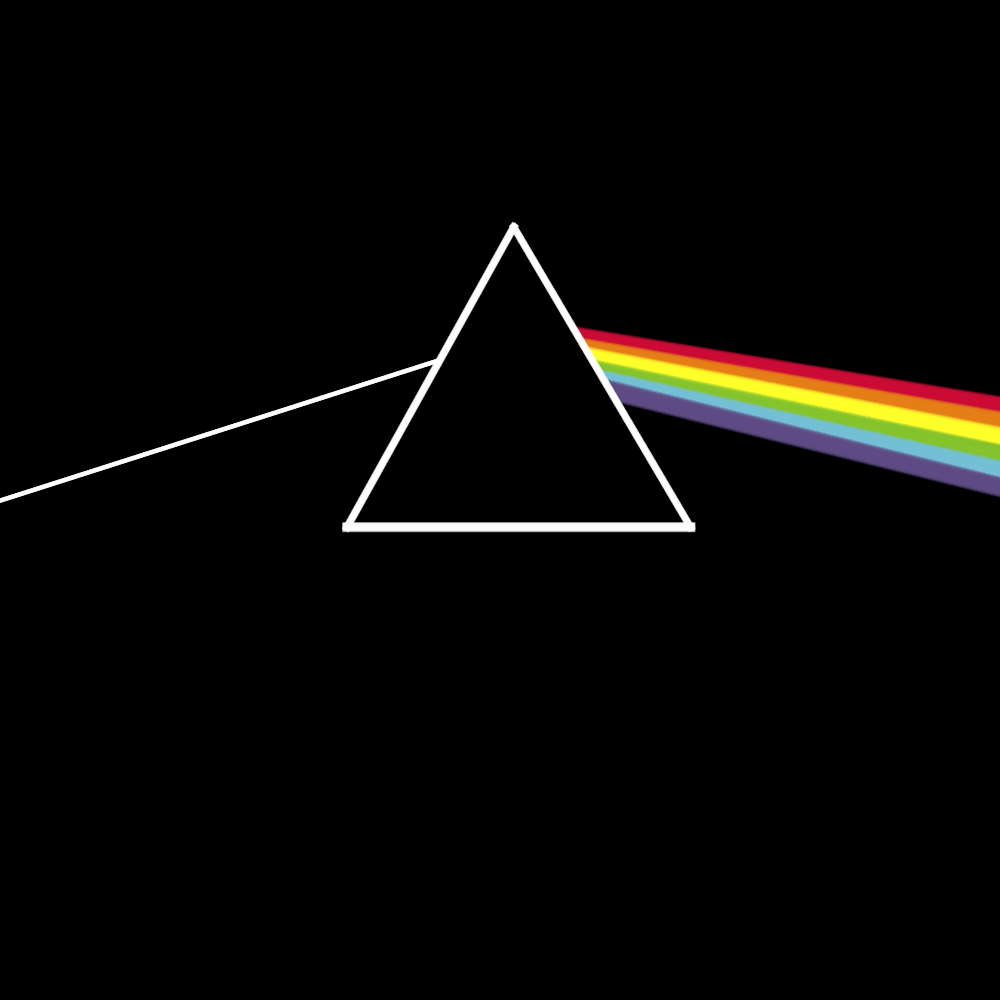
\includegraphics[width=\linewidth,scale=0.1]{images/floyd}
\caption{Pink Floyd 1000x1000 pixel rendering showing anti-aliasing}
\label{figure:floyd}
\end{figure}

\end{document}

